\section{Dáta v doméne CQA systémov}

Experimenty s personalizáciou informačných bulletinov budeme realizovať na platforme Stack Exchange, ktorá patrí medzi
najpopulárnejšie CQA systémy súčasnosti a tvorí ju viac ako 160 samostatných komunít zameraných na rôzne oblasti.

Experimenty plánujeme vykonávať nad dátami z komunity \textit{Software Engineering}\footnote{\url{http://softwareengineering.stackexchange.com}},
nakoľko je táto komunita zameraná na doménu, v ktorej máme hlbšie vedomosti a teda vieme lepšie posúdiť správnosť
odporúčania v tejto doméne. Navrhnuté riešenie však nebude špecifické pre túto komunitu, našim cieľom je naopak vytvoriť
metódu, ktorú bude možné nasadiť v rámci celej platformy Stack Exchange, rovnako ako na iných CQA systémoch s podobnou
štruktúrou.

Platforma Stack Exchange pravidelne zverejňuje kompletné archívne dáta zo všetkých komunít vo forme XML výstupov reflektujúcich
entity systému. Tieto dáta plánujeme využiť v prvotnej fáze experimentov na vytvorenie základných modelov.
Pre následné zdokonaľovanie modelov, ako aj zabezpečenie aktuálnosti použitých dát budeme využívať verejné API poskytované
platformou Stack Exchange.

\subsection{Charakteristika dát}

\subsubsection{Archívne dáta}
Dáta v dátovom archíve platformy Stack Exchange\footnote{\url{http://archive.org/details/stackexchange}} sú pravidelne
aktualizované a obsahujú kompletné používateľmi vytvorené anonymizované dáta zo všetkých komunít platformy.
Všetky tieto dáta sú verejne dostupné pod licenciou \emph{Creative Commons Attribution-ShareAlike 3.0 Unported}.

Štruktúra dát v archívoch je nasledovná:

\begin{my_itemize}
  \item{\textit{Badges.xml} -- Obsahuje ID používateľov, názvy odznakov a čas, kedy používateľ daný odznak získal.}
  \item{\textit{Comments.xml} -- Obsahuje všetky komentáre spolu s informáciou o ich autoroch a príspevkoch, ku ktorým sa viažu.}
  \item{\textit{Posts.xml} -- Obsahuje informácie o všetkých príspevkoch (otázkach a odpovediach) a k nim prislúchajúce značky, ako aj aktuálne znenie príspevku}
  \item{\textit{PostHistory.xml} -- Obsahuje históriu zmien jednotlivých príspevkov, ako napr. zmenu názvu, štítkov, označenie otázky za zodpovedanú a pod.}
  \item{\textit{PostLinks.xml} -- Obsahuje informácie o prepojeniach medzi príspevkami, konkrétne o duplikátoch a príbuzných príspevkoch.}
  \item{\textit{Users.xml} -- Obsahuje verejné údajé všetkých používateľov, ako sú meno, reputácia, webová stránka, počet hlasov a iné.}
  \item{\textit{Votes.xml} -- Obsahuje anonymizované informácie o hlasoch príspevkov.}
\end{my_itemize}


\subsubsection{Stack Exchange API}

API platformy Stack Exchange\footnote{\url{http://api.stackexchange.com}} poskytuje prístup ku všetkým verejným dátam
platformy v reálnom čase. API podporuje dvojúrovňový prístup k dátam.

\textbf{Obmedzenia požiadaviek}\\
Menšie aplikácie môžu využiť základnú úroveň, ktorá na používanie nevyžaduje registráciu a autentifikáciu,
no jej prístup podlieha obmedzovaniu v miere prístupu a môže z jednej IP adresy denne vykonať iba 10 000 požiadaviek na API.

V prípade, že aplikácia využívajúca API vykoná autentifikáciu používateľa, je limit 10 000 požiadaviek denne špecifický
pre každého používateľa zvlášť.

Bez ohľadu na úroveň prístupu je tiež uplatňované limitovanie na 30 požiadaviek za sekundu z jednej IP adresy, ako aj
dynamické limitovanie, ktoré spočíva v tom, že každá odpoveď API môže obsahovať parameter indikujúci počet sekúnd, koľko
má aplikácia počkať pred vykonaním ďalšej požiadavky. Tento limit musí dodržiavať každá aplikácia.

\textbf{Vlastné filtre}\\
Stack Exchange API umožňuje flexibilne špecifikovať jednotlivé atribúty, ktoré majú byť vrátené v odpovedi na požiadavku.
Táto podpora je implementovaná prostredníctvom filtrov, ktoré môže aplikácia využívajúca API vytvoriť. Každý filter môže
obsahovať (1) zoznam atribútov, ktoré majú byť prítomné, (2) atribúty, ktoré nemajú byť súčasťou odpovede a (3) základný
filter, od ktorého je daný filter odvodený.\\
Použitie filtrov umožňuje aplikáciám pokladať efektívnejšie požiadavky, ktoré vrátia iba všetky aplikáciou požadované
atribúty a nič navyše.

\textbf{Autentifikácia}\\
Autentifikácia používateľov pri použití API je implementovaná prostredníctvom otvoreného štandardu
OAuth 2.0\footnote{\url{http://oauth.net}}. Pre využívanie autentifikovaných požiadaviek v API je nutné zaregistrovať
aplikáciu v centrálnom zozname všetkých aplikácií využívajúcich API platformy Stack Exchange --
\textit{Stack Apps}\footnote{\url{http://stackapps.com}}.

\subsubsection{Rozsah dát}

Komunita \textit{Software Engineering}, ktorú budeme využívať v experimentoch pri návrhu riešenia má nasledovný rozsah:

\begin{my_itemize}
    \item{Otázky - cca 45 tisíc}
    \item{Odpovede - cca 138 tisíc}
    \item{Používatelia - cca 221 tisíc}
    \item{Pridelené odznaky - cca 405 tisíc}
    \item{Komentáre - cca 397 tisíc}
    \item{Značky - cca 1.6 tisíc}
    \item{Miera zodpovedanosti otázok - cca 94\%}
\end{my_itemize}












Model otázok bude zložený z troch nezávislých modelov, ktoré sa na otázky pozerajú z rôznych perspektív.

\begin{my_enumerate}
\item{\textbf{Kategorický model otázok}\\
Tento model reprezentuje otázku na najvyššej úrovni ako prislúchajúcu do určitých kategórií. Kategórie otázok sú v rámci
platformy Stack Exchange reprezentované ako značky (angl.~\emph{tags}). Každá otázka môže obsahovať viacero značiek, pričom
platforma identifikuje aj synonymické značky, ktoré možno chápať ako bližšie určenie kategórie.}

\item{\textbf{LDA tématický model}\\
Tento model využíva metódu latentnej Dirichletovej alokácie (angl.~\emph{Latent Dirichlet Allocation})~\cite{blei2003latent}
na určenie témy, ktorej sa daná otázka venuje. LDA vektor je vypočítaný z nadpisu a samotného textu otázky.}

\item{\textbf{Komunitný model}\\
\textit{Komunitný model} je naše pomenovanie pre model reprezentujúci komunitný faktor danej otázky. Predstavuje ho vektor
zložený z viacerých čŕt, ako napr. počet hlasov, počet odpovedí, atď. Presný zoznam použitých čŕt obsahuje
kapitola~\ref{features}. Tento model predstavuje prínos a hodnotu otázky pre komunitu.}
\end{my_enumerate}


\subsection{Model používateľov}

Model používateľa bude vytvorený prostredníctvom agregácie modelov otázok, s~ktorými používateľ v minulosti interagoval
-- či už ich pokladal, odpovedal na ne, alebo za otázku hlasoval, okomentoval ju alebo ju označil za obľúbenú.

Druh interakcie používateľa s otázkou bude mať dopad na faktor, s akým bude daná interakcia agregovaná -- menšie interakcie
(hlasovanie, komentár) budú brané do úvahy menej ako napr. odpovedanie alebo samotné položenie otázky.

S cieľom reflektovať časom sa meniace preferencie používateľa bude tiež aplikovaný faktor zmeny (angl.~\emph{decaying factor}).


\subsection{Výber odporúčaného obsahu}\label{rec-retrieval}

Pre účely zostavovania zoznamu odporúčaných otázok použijeme prístup analogický štandardným nástrojom pre vyhľadávanie
informácií (angl.~\emph{Information Retrieval Engines}). V našom prípade budú dokumentmi samotné otázky a dopytom bude
model používateľa. Pre ohodnocovanie podobnosti modelov bude použitý skalárny súčin vektorov reprezentujúcich
modely otázky a používateľa.


\subsection{Riešenie problému studeného štartu}

Pre eliminovanie problému studeného štartu (kapitola~\ref{cold-start}) z pohľadu prvotného odporúčania otázok využijeme
offline natrénovanie našich metód na archívnych dátach platformy Stack Exchange.

V prípade nových používateľov, ktorí v systéme nemajú žiadnu, alebo iba nedostatočnú aktivitu, budeme zo začiatku vytvárať
iba generický informačný bulletin podobný tomu, ktorý je používateľom k dispozícii aj v súčasnosti (kapitola~\ref{so-newsletter}).


\section{Návrh metódy diverzifikácie odporúčaní}

\textbf{Hypotéza}\\
\textit{Výberom odporúčaných otázok zo širšieho okruhu záujmu používateľa a zohľadnením ich aktuálnosti predídeme výskytu problému
filtračnej bubliny, čím dosiahneme vyššiu mieru záujmu používateľa a jeho aktivity.}

Pre účely diverzifikácie odporúčaných otázok budeme porovnávať výsledky dvoch rôznych metód diverzifikácie.

\subsection{Tematické vzorkovanie}
Metódu diverzifikácie prostredníctvom tematického vzorkovania sme navrhli nasledovne:

\begin{my_enumerate}
\item{
  Pre každého používateľa vyberieme náhodne N rôznych tém, ktoré sú pre neho relevantné. Tieto témy sa vyberú zo zoznamu
  kategórií a LDA tém z~modelu používateľa.
}
\item{
  Prostredníctvom vyššie opísaného mechanizmu (kapitola~\ref{rec-retrieval}) vyberieme pre každú takúto tému zoznam
  odporúčaní.
}
\item{
  Následne sa budú z jednotlivých zoznamov vyberať samotné položky do výsledného zoznamu odporúčaní. Pravdepodobnosť výberu
  otázky z konkrétneho zoznamu bude proporčná k relevancii tejto témy pre daného používateľa.
}
\item{
  Pravidlá pre výber konkrétnych otázok z jednotlivých zoznamov zatiaľ nešpecifikujeme. Pre účely zvýšenia diverzity však
  nepredpokladáme jednoduchý výber podľa poradia v rámci zoznamu, ale aplikovanie inej distribúcie, prípadne náhodný výber.
}
\end{my_enumerate}

Proces tematického vzorkovania ilustruje schéma na obrázku~\ref{fig:tematic-sampling}.

\begin{figure}[H]\begin{center}
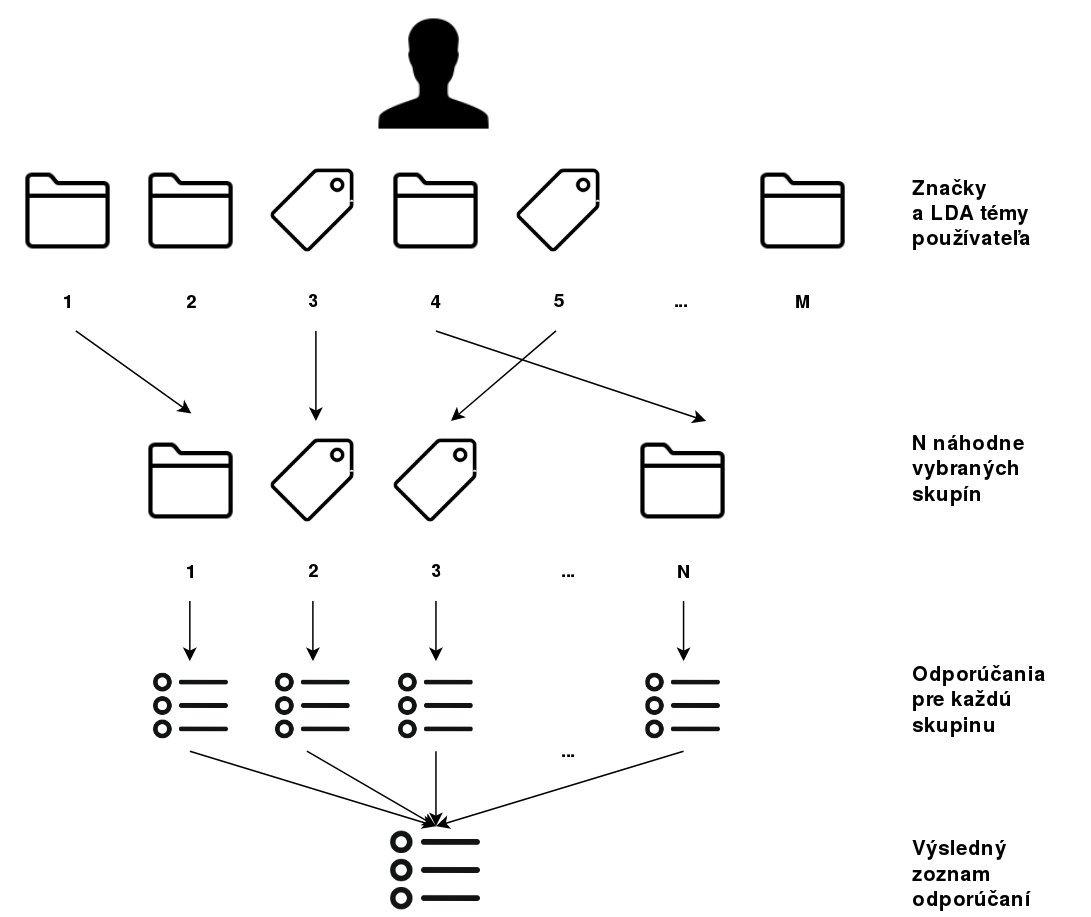
\includegraphics[scale=0.27]{diversity-diagram}
\caption{Schéma metódy diverzifikácie odporúčaní tematickým vzorkovaním.\label{fig:tematic-sampling}}\end{center}
\end{figure}


\subsection{Proporčná diverzifikácia}
Táto metóda diverzifikácie je vo svojej podstate jednoduchšia a priamočiarejšia ako tematické vzorkovanie. Spočíva
vo výbere N najrelevantnejších tém, pričom témy sú definované rovnako, ako v prípade tematického vzorkovania.
Samotné otázky zo zoznamov jednotlivých tém sú vyberané od vrchu podľa ich ohodnotenia.


\section{Výber čŕt pre použitie v metódach}\label{features}

\begin{my_itemize}
  \item Črty otázok
  \begin{my_itemize}
    \item Nadpis otázky
    \item Text otázky
    \item Značky priradené k otázke
    \item Dátum poslednej zmeny
    \item Počet hlasov - skóre
    \item Počet zobrazení
    \item Počet označení za obľúbenú
    \item Má/nemá akceptovanú odpoveď
    \item Počet odpovedí
    \item Súhrnný počet komentárov (počet komentárov na otázke aj odpovediach)
    \item Počet zmien v otázke
    \item Reputácia autora otázky
    \item Reputácia autora akceptovanej odpovede
  \end{my_itemize}
  \item Črty používateľov
  \begin{my_itemize}
    \item Reputácia používateľa
    \item Počet kladných hlasov
    \item Počet záporných hlasov
    \item Počet položených otázok
    \item Počet komentárov
    \item Počet poskytnutých odpovedí
    \item Dátum registrácie
    \item Dátum poslednej aktivity
  \end{my_itemize}
\end{my_itemize}

\section{Metriky hodnotenia výsledkov}

Pre overovanie výsledkov experimentov budeme používať tieto metriky:

\textbf{Precision@N}\\
Presnosť (angl.~\emph{Precision}), alebo tiež \textit{pozitívna predikčná hodnota} je metrika reprezentujúca pomer relevantných
dokumentov z celkového zoznamu. Štandardne sa presnosť počíta ako pomer z celého zoznamu dokumentov, no v oblasti
odporúčania a vyhľadávania informácií je často vhodnejšou odvodená metrika \textit{Precision@N}, ktorá určuje, aká časť
z prvých N dokumentov v zozname je relevantná.

\textbf{nDCG}\\
\textit{Normalized Discounted Cumulative Gain} je metrika kvality ohodnocovania často používaná na meranie efektívnosti
odporúčania. DCG meria užitočnosť dokumentov na základe ich pozície vo výslednom zozname. Užitočnosť dokumentov sa akumuluje
od konca zoznamu, pričom najvyššiu užitočnosť majú dokumenty na začiatku zoznamu~\cite{Jrvelin2002}.

\textbf{CTR}\\
Miera preklikov (angl.~\emph{Click-through Rate}) je metrika často využívaná v spojitosti s informačnými bulletinmi.
Táto metrika vyjadruje počet úspešných kliknutí na odkaz v informačnom bulletine.

Okrem CTR plánujeme v súvislosti s interakciou používateľa s informačným bulletinom merať aj počet impresií,
teda zobrazení informačného bulletinu, ako aj počet konverzií, teda podiel prípadov, kedy kliknutie na niektorú z otázok
v informačnom bulletine viedlo k aktivite používateľa na tejto otázke -- či už hlasovanie, odpovedanie alebo pridanie komentáru.


\section{Návrh overenia metód}

Nami navrhnuté metódy personalizovaného odporúčania a diverzifikácie odporúčaného obsahu budeme overovať prostredníctvom
online nekontrolovaného experimentu na používateľoch z komunity \textit{Software Engineering} platformy Stack Exchange.

Tento online experiment bude mať formu pravidelne rozposielaného informačného bulletinu, na ktorého odoberanie sa budú
môcť prihlásiť všetci používatelia z tejto komunity.

Účinnosť zvolených metód diverzifikácie odporúčaní budeme vyhodnocovať prostredníctvom A/B testovania, pričom používateľov
rozdelíme na tri skupiny:
\begin{my_enumerate}
    \item{Kontrolná skupina -- odporúčania nebudú diverzifikované}
    \item{Skupina A -- využitie metódy tematického vzorkovania}
    \item{Skupina B -- využitie metódy proporčnej diverzifikácie}
\end{my_enumerate}

Dôležitým predpokladom pre úspešnosť online experimentu bude získať dostatočnú reprezentatívnu vzorku používateľov
ochotných byť súčasťou experimentu. V~prípade, že by sa nám nepodarilo osloviť dostatočný počet používateľov, plánujeme
vykonať kontrolovaný offline experiment na vzorke archívnych dát.


